\documentclass{standalone}
\usepackage[svgnames]{xcolor}
\usepackage{tikz}
\usetikzlibrary{arrows.meta}
\begin{document}
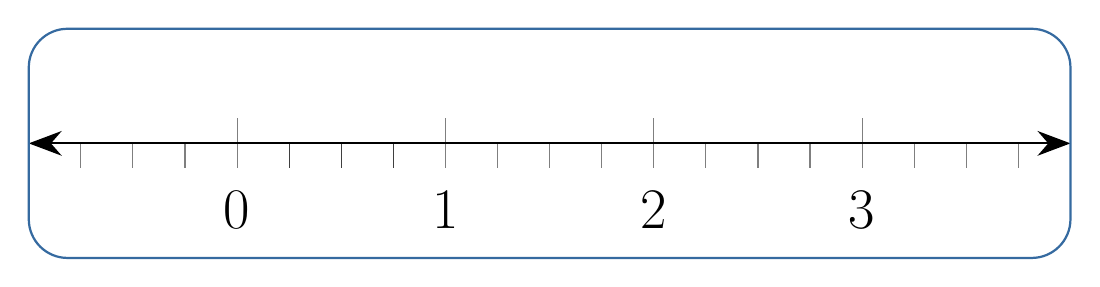
\begin{tikzpicture}[x=1.04166666666667in,y=1.43229166666667in]

\tikzset{
	>={Stealth[scale=1.8]},
	clip even odd rule/.code={\pgfseteorule},
	inverse clip/.style={ clip,insert path=[clip even odd rule]{
		(-1,-0.4) rectangle (4,0.4) }
	}
}
\definecolor{borderblue}{HTML}{356AA0}
\definecolor{fillpurple}{HTML}{A384E5}
\pgfdeclarelayer{background}
\pgfdeclarelayer{foreground}
\pgfsetlayers{background,main,foreground}
\begin{pgfonlayer}{background}
	\fill[white,rounded corners=14pt]
	(-1,-0.4) rectangle (4,0.4);
\end{pgfonlayer}
\huge
\draw[<->,thick] (-1,0) -- (4,0)
node[above left,outer sep=2pt]{\(\)};
\foreach \x/\label in {0/0,1/1,2/2,3/3}{\draw[thin, opacity = 0.5] (\x,9pt) -- (\x,-9pt) node[baseline, yshift = -15pt, opacity = 1]{\(\label\)};}
\foreach \x in {-0.75,-0.5,-0.25,0.25,0.5,0.75,0.25,0.5,0.75,1.25,1.5,1.75,2.25,2.5,2.75,3.25,3.5,3.75}{\draw[thin, opacity = 0.5] (\x,0) -- (\x,-9pt);}
\draw[borderblue,rounded corners=14pt,thick] (-1,-0.4) rectangle (4,0.4);
\begin{pgfonlayer}{foreground}
\clip[rounded corners=14pt] (-1,-0.4) rectangle (4,0.4);
\end{pgfonlayer}
\begin{pgfonlayer}{background}
\end{pgfonlayer}
\end{tikzpicture}
\end{document}
